\documentclass[12pt]{article}
\input{.house-style/preamble.tex}
\usepackage{float}
\usepackage{tikz}
\usetikzlibrary{arrows.meta}
\hypersetup{
  pdftitle={From Aggregate Scores to Warranted Inference in AGI Evaluation},
  pdfkeywords={AGI evaluation, validity, projectibility, robustness, transportability}
}
\setlength{\headheight}{14pt}
\setlength{\emergencystretch}{1.5em}
\fancypagestyle{appendixmixed}{%
  \fancyhf{}%
  \fancyhead[L]{\small\scshape Conclusion and Formal Sanity Check}%
  \fancyhead[R]{\small\thepage}%
  \renewcommand{\headrulewidth}{0pt}%
}

\newcommand{\ins}{\mathrm{INS}}
\newcommand{\wtd}{\mathrm{WTD}}
\newcommand{\wtl}{\mathrm{WTL}}

\title{From Aggregate Scores to Warranted Inference\\in AGI Evaluation}
\author{Brett Reynolds \orcidlink{0000-0003-0073-7195}\thanks{I used ChatGPT 5, Claude Sonnet 4.5, and Gemini Pro 2.5 extensively in drafting and revising the paper. I reviewed, edited, and approved all the material and take full responsibility for the final text and conclusions. \href{mailto:brett.reynolds@humber.ca}{brett.reynolds@humber.ca}}\\
Humber Polytechnic \& University of Toronto}
\date{}

\begin{document}

\maketitle

\begin{abstract}
Finite multidomain batteries are routinely used to support inferences about untested tasks, contexts, systems, and future behaviour. Precision within a standardized evaluation universe doesn't establish extrapolation to a declared target; more observations from the same narrowed universe don't repair underrepresentation. Aggregate stability can also coexist with offsetting item changes, while a change-based tail statistic can miss severe failures stable across conditions. The question is which compressed distinctions matter to a bounded source--target inference or decision. I use \term{projectibility} for the target-indexed support that observations provide for such an inference beyond score construction, as one part of a broader validity argument.

I develop an evaluation discipline with three moves. First, declare a bounded projection, including its source and target populations, bearer, intervention and temporal ranges, probability measure, decision criterion, evidential test, and responsible parties. Second, when a paired multidomain comparison bears on that projection, use a five-part descriptive module: domain-profile correlation, signed level change, item instability, worst-tail degradation, and absolute worst-tail loss. Third, test the projection using untouched evidence that matches the claimed item, context, system, or temporal range. Causal claims require interventions against rival routes; decision use requires declared objectives, tradeoffs, and constraints.

Commensurability, compensability, and projectibility are separate questions about aggregate interpretation and use; interpretable scores, predictive models, and decision rules are distinguished. Developer and deployer responsibilities are allocated across the source--target relation; retention, feedback, and component dependence receive separate controls. The empirical companion reanalyses 32 released model--benchmark cells and uses known-truth simulations to demonstrate paired-condition distinctions and conditional estimator behaviour, including why pseudo-null-adjusted and split-tail estimates aren't interchangeable. It supplies no external projection target. The framework specifies how to test bounded target-indexed inferences beyond score construction; wider ranges require new tests, and no finite battery warrants unrestricted AGI generality.
\end{abstract}

\noindent\textbf{Keywords:} AGI evaluation; validity; projectibility; robustness; transportability

\section{The Inferential Overreach of AGI Scores}\label{sec:problem}

Multidomain evaluations are often invoked to support inferences or decisions without evidence that the distinctions compressed by their aggregate scores are irrelevant to those uses. Standardization fixes prompts, scoring, and conditions so that repeated evaluation answers a stable question. It also narrows the universe represented by the score. When fixed facets vary in the intended target domain, reliability within the standardized universe can increase while extrapolation weakens \parencites[22--31]{kane2013validating}[132--135]{brennan2001generalizability}. More observations from the narrowed universe leave systematic underrepresentation of the target intact.

\textcite{zhang2026illusionRobustness} supply a controlled AI example. They add task-irrelevant context to benchmark items and find that aggregate accuracy often moves little even when many item-level response probabilities move in opposite directions. Their adjusted estimates reach 13.6\% for mean absolute item change and 53.2\% for worst-decile degradation across the reported model--benchmark cells. The affected examples are also largely model-specific.

A stable mean is compatible with unchanged items, balanced improvements and degradations, or a persistent set of serious failures. Those states may support different predictions and decisions. The declared target determines the useful granularity.

Interpreting a finite evaluation as evidence of general capability widens the gap. \textcite{raji2021whole} argue that broad benchmark claims routinely outrun the contextual tasks used to construct them. \textcite{hendrycks2025agi} respond to part of this problem with a revisable ten-domain task framework informed by Cattell--Horn--Carroll (CHC) theory. They warn that a total can conceal bottleneck failures and recommend reporting the domain profile, the vector of domain scores, alongside it.

The profile preserves distinctions that a total erases, but it still compresses item changes and tails, and its domain structure may not transfer across systems. Neither total nor profile establishes which inferences the task framework supports beyond its construction.

Claims made under the label AGI are typically open-ended: their intended range isn't exhausted by an enumerated task battery. A study should therefore declare the bounded source--target claim it addresses, preserve distinctions potentially relevant to that claim, and test the projection with evidence withheld from score construction. Aggregates can describe their construction samples; broader uses require matching warrants. Success on one projection may motivate a wider declaration, but warrants don't automatically compose into unrestricted generality.

\section{From Observations to Declared Projections}\label{sec:projection}

On the interpretation-and-use account adopted here, validity attaches to proposed score interpretations and uses, not to a test in isolation \citep{messick_1989_validity,messick1995Validity,kane2013validating}.

For \textcite[85--86, 94--98]{Goodman1983}, projectibility is historical and practice-relative: it depends on past actual projections and on entrenchment produced by linguistic use. \textcite[136--141]{boyd1991} treats projectability judgments as empirically revisable in light of background theory and, for inductive or explanatory categories, answerable to causal structure. I use \term{projectibility} for the evidential status of a declared source--target inference beyond the observations used to construct a score. The procedure developed here operationalizes that status for declared evaluation targets. The evaluator chooses the target; matching evidence determines whether the projection succeeds.

In the argument-based approach, \textcite{kane2013validating} evaluates the assumptions connecting observed responses, scores, a universe of admissible observations, a target domain, and score use. Projectibility names the family of beyond-construction links in that sequence. Generalization to an admissible test universe, extrapolation to a broader target domain, transport across contexts or systems, and temporal prediction require different evidence.

Table~\ref{tab:projection_relations} separates six inferential relations from decision use. Inferential relations concern what observations support beyond their construction; decision use combines projectible estimates with a declared loss, utility, or constraint.

\begin{table}[H]
\centering\small
\caption{Inferential relations, decision use, and evidence that could warrant them.}\label{tab:projection_relations}
\begin{tabular}{@{}>{\raggedright\arraybackslash}p{0.25\linewidth}
                    >{\raggedright\arraybackslash}p{0.29\linewidth}
                    >{\raggedright\arraybackslash}p{0.37\linewidth}@{}}
\toprule
Claim or use & Declared range & Matching evidence \\
\midrule
Observed responses to test universe & Admissible item, template, and replicate universe & Sampling or cluster holdout from the declared test frame \\
Test universe to target task domain & Intensionally specified tasks and operating conditions & External task or episode sample from the declared target frame \\
One context to another & Realizations or perturbation families & Hold out realizations, or entire families for the stronger claim \\
One system population to another & Models, lineages, or configurations & Hold out the corresponding systems rather than near-identical versions \\
Present to future behaviour & Sessions, releases, or deployment periods & Chronological validation at the stated horizon \\
Behaviour to causal explanation & Mechanisms and rival routes & Mechanistic intervention and controls for alternative causes \\
Score to decision & Actions and consequences & Independent calibration in the target setting plus a declared loss, utility, or constraint \\
\bottomrule
\end{tabular}
\end{table}
\thispagestyle{fancy}

For any row in Table~\ref{tab:projection_relations}, an evaluator should register a \term{projection declaration} for a bounded source--target claim before calculation:

\begin{enumerate}
\item \textbf{Claim and source--target relation}: the outcome, interpretation, or explanation to be inferred, the source evaluation universe, and the bounded target range
\item \textbf{System population}: the model families, versions, configurations, settings, and users in scope
\item \textbf{Task population}: the intensional task specification or admissibility rule and its sampling frame
\item \textbf{Bearer and unit}: a base model, stateful agent, or deployed model--tool--retrieval composite, together with the observational unit
\item \textbf{Intervention range}: the perturbation families and realizations over which the claim is meant to hold
\item \textbf{Time horizon}: immediate, delayed, or later deployment behaviour
\item \textbf{Risk measure}: the item, episode, or realization bearing loss and its target-population probability measure
\item \textbf{Decision criterion}: the objectives, consequences, preferences or loss, applicable constraints, and action threshold
\item \textbf{Evidential test and responsibility}: the holdout unit or other evidence that could support or defeat the claim, who supplies the source evidence, and who can perform target-specific testing
\end{enumerate}

The source evaluator and target decision-maker may be different organizations. Dividing the work doesn't remove the source--target link that needs warrant.

A separate sampling audit records what generated the observations: model and version, item, domain, perturbation family and realization, response replicate, scorer, and time. Facets may be crossed or nested, and their levels may be fixed or sampled. Generalizability theory provides the established vocabulary of an admissible universe, multiple facets, and a decision-specific measurement design \citep{brennan2001generalizability}. The analysis below combines that machinery with signed, paired, and tail-sensitive descriptions.

The same interaction may be error for one projection and signal for another. A system-by-item-by-context component is error for a context-invariant ranking but signal for predicting context-specific risk. Zhang et al.'s model-specific item changes show why the classification has to follow the target.

A system \enquote{lineage} is an operational dependency group defined by declared provenance, training, distillation, shared components, or data dependence rather than by a family label alone.

Consider a running release decision. A committee wants to predict serious task loss for a deployed agent when it encounters a previously unseen family of irrelevant contexts over the next release cycle. The system population is the product lineage, the item population is the declared deployment-task frame, the bearer is the full agent, the outer holdout is a later version crossed with a held-out context family, and the release rule includes an absolute tail-loss constraint. A random item split within familiar contexts wouldn't test that projection.

Transporting a causal effect between populations requires assumptions about which mechanisms change and which remain invariant \citep{pearlBareinboim2014externalValidity}. Figure~\ref{fig:selection_diagram} uses the corresponding selection-diagram notation to show the mismatch between the intended target and a random item split; the framework below concentrates on predictive and decision claims.

\begin{figure}[H]
\centering
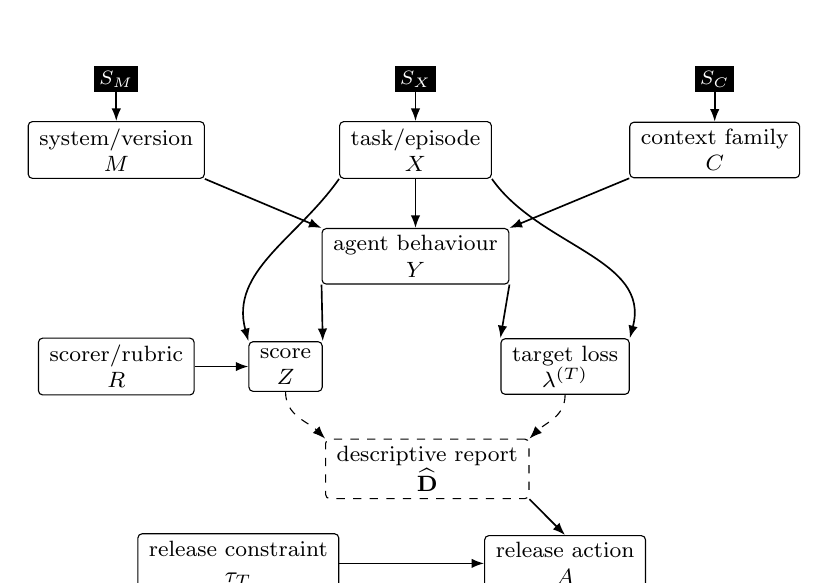
\begin{tikzpicture}[
  x=1cm,
  y=1cm,
  >=Latex,
  var/.style={draw, rounded corners=1.5pt, align=center, font=\footnotesize,
    inner xsep=4pt, inner ysep=2.5pt},
  sel/.style={draw, rectangle, fill=black, text=white, font=\scriptsize,
    inner sep=1.5pt},
  report/.style={var, dashed},
  causal/.style={-{Latex[length=1.6mm]}, semithick},
  construction/.style={-{Latex[length=1.6mm]}, dashed}
]
\node[var] (m) at (-3.8,0) {system/version\\\(M\)};
\node[var] (x) at (0,0) {task/episode\\\(X\)};
\node[var] (c) at (3.8,0) {context family\\\(C\)};
\node[sel] (sm) at (-3.8,.9) {\(S_M\)};
\node[sel] (sx) at (0,.9) {\(S_X\)};
\node[sel] (sc) at (3.8,.9) {\(S_C\)};
\node[var] (y) at (0,-1.35) {agent behaviour\\\(Y\)};
\node[var] (r) at (-3.8,-2.75) {scorer/rubric\\\(R\)};
\node[var] (z) at (-1.65,-2.75) {score\\\(Z\)};
\node[var] (ell) at (1.9,-2.75) {target loss\\\(\lambda^{(T)}\)};
\node[report] (d) at (.15,-4.05) {descriptive report\\\(\widehat{\mathbf D}\)};
\node[var] (tau) at (-2.25,-5.25) {release constraint\\\(\tau_T\)};
\node[var] (a) at (1.9,-5.25) {release action\\\(A\)};
\draw[causal] (sm) -- (m);
\draw[causal] (sx) -- (x);
\draw[causal] (sc) -- (c);
\draw[causal] (m.south east) -- (y.north west);
\draw[causal] (x.south) -- (y.north);
\draw[causal] (c.south west) -- (y.north east);
\draw[causal] (r.east) -- (z.west);
\draw[causal] (y.south west) -- (z.north east);
\draw[causal] (y.south east) -- (ell.north west);
\draw[causal] (x.south west) to[out=235,in=105] (z.north west);
\draw[causal] (x.south east) to[out=305,in=75] (ell.north east);
\draw[construction] (z.south) to[out=270,in=135] (d.north west);
\draw[construction] (ell.south) to[out=270,in=45] (d.north east);
\draw[causal] (d.south east) -- (a.north);
\draw[causal] (tau) -- (a);
\end{tikzpicture}
\caption{Selection diagram for the running release example. Filled \(S\)-nodes mark source--target differences permitted in the system, task, and context mechanisms or marginals. The intended holdout changes the system version and context family; a random item split varies only tasks under familiar systems and contexts. Solid arrows state episode-level causal or scoring assumptions, whereas dashed arrows denote construction of the report.}\label{fig:selection_diagram}
\end{figure}

\section{Distinctions Lost under Aggregation}\label{sec:profile}

Aggregation collapses distinctions at several levels: a stable domain mean can coexist with item-level churn, a stable ten-domain profile with a sharp failure in a narrow construction or subprocess, and a stable average across models with family-specific failure sets.

\subsection{Data Structure and Three Estimand Modes}\label{ssec:setup}

Counting response rows as independent observations would generally be wrong; the independent unit follows the projection declaration.

To keep the definitions readable, fix a system, time, scorer protocol, and perturbation realization. Let domains be indexed by \(g=1,\ldots,G\), items within domain \(g\) by \(i=1,\ldots,N_g\), and conditions by \(c\), with baseline \(0\) and perturbation \(p\). Let \(s_{igc}\in[0,1]\) be the item score. In a sequential-agent evaluation, an item may be a complete task episode or trajectory, provided its score and target loss are defined at that level. Define
\[
\delta_{igp}=s_{igp}-s_{ig0},
\qquad
a_{gc}=\frac{1}{N_g}\sum_{i=1}^{N_g}s_{igc},
\]
and let \(\mathbf a_c=(a_{1c},\ldots,a_{Gc})\).

The same symbols support three different estimands. With deterministic decoding on a fixed paired set, the quantities below are exact descriptions of that set. Under a declared stochastic generation and scoring protocol, \(s_{igc}\) is an expected score estimated from repeated responses and, when relevant, scorers. Inference to an item, context, system, or time population also requires sampling or holdout from that declared universe. Repetition within an item doesn't create a representative item sample.

If item inclusion probabilities differ, population means require design weights and a \(q\)-tail should represent \(q\) of the target-population mass. The unweighted formulas below use the empirical item measure, so they describe a fixed equally weighted set or an equal-probability sample.

For the paired-condition design, Table~\ref{tab:descriptions} gives the descriptive module used here; reports using it should retain the raw domain profiles and item-change distributions alongside the summaries.

\begin{table}[tbp]
\centering\small
\caption{Distinct descriptions in a paired-condition report before target-specific testing.}\label{tab:descriptions}
\begin{tabular}{@{}>{\raggedright\arraybackslash}p{0.16\linewidth}
                    >{\raggedright\arraybackslash}p{0.25\linewidth}
                    >{\raggedright\arraybackslash}p{0.50\linewidth}@{}}
\toprule
Output & Granularity & Question answered \\
\midrule
\(r_p\) & Domain profile & How strongly were the centred, scaled domain profiles linearly associated? \\
\(L_{gp},L_p\) & Domain and overall level & Did average performance rise or fall? \\
\(\ins_{gp}\) & Items within a cell & How much two-sided paired item change occurred? \\
\(\wtd_{q,gp}\) & Change tail & How large was mean degradation in the worst-changing \(q\)-fraction? \\
\(\wtl^{(T)}_{q,gc}\) & Absolute loss tail & How large was target-specific loss in the worst-loss \(q\)-fraction? \\
\bottomrule
\end{tabular}
\end{table}

\subsection{Profile Correlation and Signed Level}\label{ssec:profile_level}

For nonconstant profiles, report Pearson correlation directly:
\[
r_p=\operatorname{corr}_g(\mathbf a_0,\mathbf a_p)\in[-1,1].
\]
A high \(r_p\) establishes only strong linear association between the centred, scaled profiles. Any positive affine transformation of the profile can yield \(r_p=1\), even when level or spread changes.

With ten fixed domains, \(r_p\) is a descriptive summary of those ten estimated means. Resampling items within domains propagates uncertainty in the means, but not uncertainty in the choice of domains. Correlation is undefined when either profile has zero variance and degenerates to \(\pm1\) with only two nonconstant domains. Reports should publish the profiles and their spreads; a preregistered centred distance or rank correlation may supplement \(r_p\) when it better matches the target.

Signed domain and overall changes are
\[
L_{gp}=a_{gp}-a_{g0},
\qquad
L_p=\frac{1}{G}\sum_{g=1}^{G}L_{gp}.
\]
They lie in \([-1,1]\) for unit-interval scores. The equal-domain mean describes an equally weighted domain set; alternative domain or deployment weights encode different scales and target mixtures and have to be labelled and justified.

\subsection{Item Instability and Directional Components}\label{ssec:item_instability}

Signed change can cancel within a domain. Mean absolute paired change is
\begin{equation}\label{eq:ins}
\ins_{gp}=\frac{1}{N_g}\sum_{i=1}^{N_g}|\delta_{igp}|\in[0,1].
\end{equation}
Its directional components are
\[
F^+_{gp}=\frac{1}{N_g}\sum_i(\delta_{igp})_+,
\qquad
F^-_{gp}=\frac{1}{N_g}\sum_i(-\delta_{igp})_+.
\]
Here \(F^+\) is mean positive change and \(F^-\) is mean negative change, recorded as a nonnegative magnitude. For deterministic binary scores, these are the incorrect-to-correct and correct-to-incorrect transition proportions. The identities
\[
L_{gp}=F^+_{gp}-F^-_{gp},
\qquad
\ins_{gp}=F^+_{gp}+F^-_{gp}
\]
make cancellation explicit and imply \(|L_{gp}|\leq\ins_{gp}\).

\subsection{Worst-Tail Degradation}\label{ssec:wtd}

Choose \(q\in(0,1]\) and a minimum tail count before inspecting results. Let \(m_g=\lceil qN_g\rceil\), and order paired changes from smallest to largest. Define
\begin{equation}\label{eq:wtd}
\wtd_{q,gp}
=-\frac{1}{m_g}\sum_{\ell=1}^{m_g}\delta_{(\ell)gp}
\in[-1,1].
\end{equation}
WTD is a finite-sample expected-shortfall analogue applied to the loss \(-\delta\) \citep{acerbiTasche2002expectedShortfall,rockafellarUryasev2002cvar}. Because the ceiling makes the empirical tail mass \(m_g/N_g\), the selected set is exactly a \(q\)-tail only when those quantities coincide.

A positive WTD indicates mean deterioration among the worst-changing items. A negative value means that even the selected lower tail improved on average. WTD measures signed worst-tail change; consequences enter through the target-specific loss defined below.

For a deployment-weighted target, the analogous statistic orders items or episodes under their declared probabilities, includes only \(q\) of the target mass (fractionally at the cutoff when needed), and averages with those probabilities. A deployment interpretation requires declared probabilities rather than item resemblance.

\subsection{Absolute Worst-Tail Loss}\label{ssec:wtl}

A change statistic misses a stable serious failure. If the same safety-critical items are failed at baseline and under perturbation, their \(\delta_{igp}\) values are zero, so both INS and WTD can be zero. The running release decision still needs an absolute loss constraint.

For target \(T\), declare an item loss \(\lambda^{(T)}_{igc}\in[0,1]\) that incorporates the response, reference outcome, and any consequence severity relevant to the decision. Because WTL averages this quantity, differences on its scale have to carry the intended loss meaning \citep{KeeneyRaiffa1993}. Ordinal hazard classes should remain separate strata or define constraints rather than be averaged as if their labels were cardinal. Order condition-specific losses from largest to smallest and define
\begin{equation}\label{eq:wtl}
\wtl^{(T)}_{q,gc}
=\frac{1}{m_g}\sum_{\ell=1}^{m_g}\lambda^{(T)}_{[\ell]gc}
\in[0,1].
\end{equation}

Report condition-specific WTL levels as primary and their difference as secondary. A binary \(1-\text{correctness}\) loss is inadequate when consequences differ across items. If loss isn't normalized, report it in its natural units; a deployment-facing WTL also uses the declared episode probabilities rather than equal item weights.

A hard WTL threshold prevents compensation by a good mean or profile, but WTL still averages losses within its selected tail. Other tail members can dilute a single red-line failure. Event-specific prohibitions or a maximum-loss constraint are the appropriate form when no within-tail tradeoff is allowed.

\subsection{Estimation, Selection, and Multiplicity}\label{ssec:uncertainty}

With stochastic generation or scoring, absolute values create a positive response-sampling floor, while selecting the worst observed tail selects noise. The positive-part directional components \(F^+\) and \(F^-\) inherit the same floor. Following \textcite{zhang2026illusionRobustness}, baseline-only pseudo-null contrasts should reproduce the real response counts. Reports should show the raw statistic, mean pseudo-null contribution, untruncated adjusted value, and uncertainty, and should name any split-sample sign-selection procedure. Each procedure targets a different finite-sample quantity; unbiased recovery of latent instability requires additional assumptions.

Tail selection and estimation should use disjoint response splits when item changes or losses are noisy. Cross-fitting targets the latent effect of the selected set without reusing the same response noise; that estimand may differ from the latent population tail. Deterministic fixed-set descriptions have no response-sampling contribution to remove, although uncertainty about new items or contexts remains.

Resampling and holdout units should follow the projection declaration. Preserve paired items, shared baselines, perturbation realizations, scorers, and model lineage. An item bootstrap conditional on fixed domains and perturbations estimates item-sampling uncertainty within those fixed facets; claims about new domains or perturbation families require corresponding outer holdouts. When a descriptive report contains many cells or tail fractions, distinguish cellwise from simultaneous uncertainty and state how selection or multiplicity is controlled.

These estimands presuppose a sound benchmark. Disaggregation can't resolve ambiguous items or an ill-designed perturbation. Annotation quality, statistical power, construct coverage, and the invariant property under stress testing have to be justified independently \citep{bowmanDahl2021benchmarking}.

\subsection{A Multilevel Descriptive Report}\label{ssec:no_scalar}

Each quantity answers a distinct question; the framework assumes no single latent robustness variable behind them. A high \(r_p\) with negative \(L_p\) means that the centred, scaled profiles remained linearly associated while level fell. Near-zero \(L_{gp}\) with high INS means that changes cancelled. High WTD localizes degradation in a change tail, while high WTL can reveal stable absolute loss even when every change statistic is zero.

When this paired-condition module is used, its primary output is a multilevel descriptive report indexed by system, domain, and perturbation. A scalar may summarize the construction sample when its operation, scale, and weights are explicit. Any warrant established for a score interpretation, predictive model, or decision rule is limited to the declared target and the population represented by its outer evidence.

\section{Empirical Demonstration and Estimator Checks}\label{sec:demonstration}

The \href{https://github.com/BrettRey/agi-evaluation-hpc/tree/master/analysis}{empirical companion} analyses released trial-level outputs from \textcite{zhang2026illusionRobustness} and known-truth simulations. It reproduces the distinction between aggregate change and paired item instability, compares raw, pseudo-null-adjusted, and split-sample tail estimators, distinguishes change tails from absolute loss tails, and probes profile correlation when between-domain spread is low.

\begin{figure}[!t]
\centering
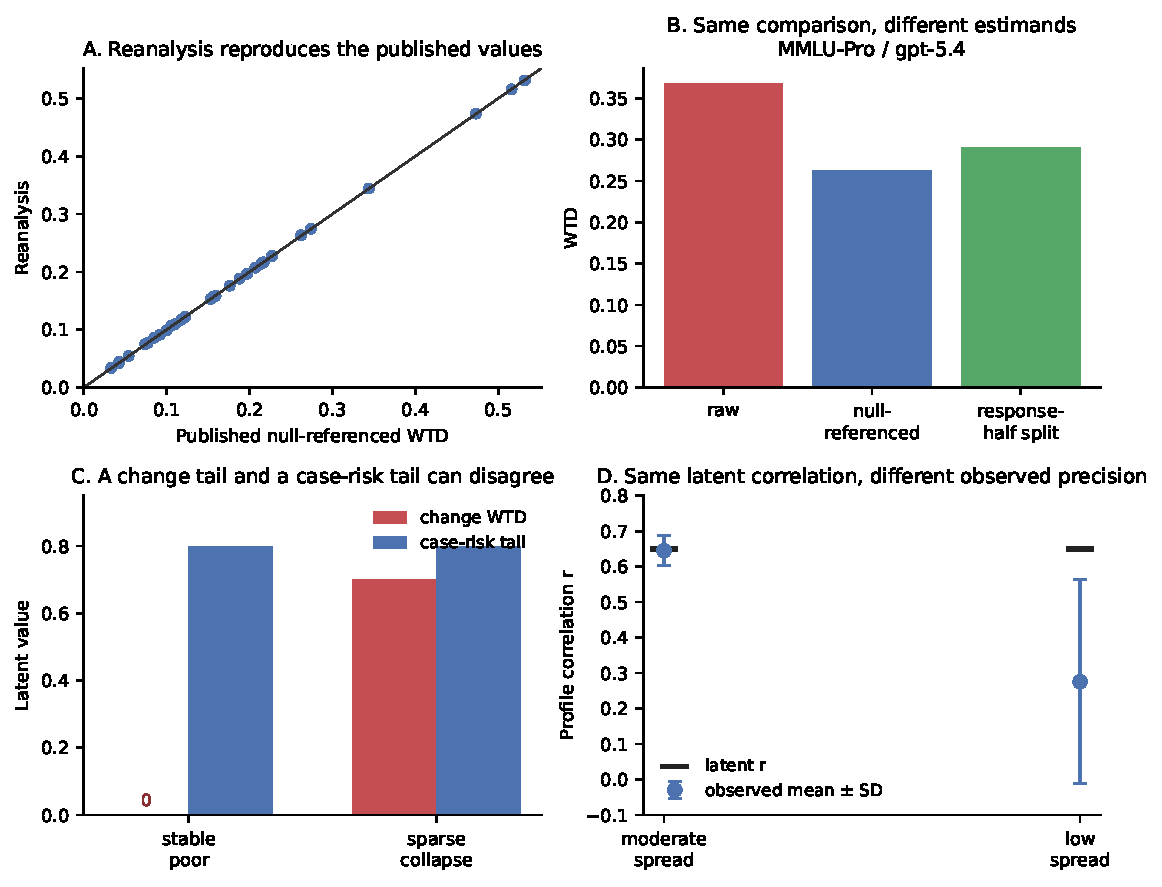
\includegraphics[width=0.94\linewidth]{analysis/outputs/section5_evidence.pdf}
\caption{Released-output reproduction and known-truth checks. (A) Recomputed adjusted WTD for all 32 cells against the rounded published values. (B) Raw, pseudo-null-adjusted, and held-out split WTD for MMLU-Pro--gpt-5.4; the latter two estimate different estimands. (C) A stable-poor simulation has zero latent WTD but .80 absolute worst-decile loss. (D) With ten domains and latent \(r=.65\), correlation estimation remains accurate at moderate profile spread but attenuates under low spread. Full settings and numerical outputs are in the empirical companion.}\label{fig:empirical_checks}
\end{figure}

\subsection{Released-Trial Reanalysis}\label{ssec:zhang_reanalysis}

The released design crosses four benchmarks with eight models and supplies 20 baseline and 20 context trials for every item in each of the resulting 32 cells. The reanalysis uses those responses rather than attempting to recreate outputs from proprietary model versions. The companion pins the preprint version, repository commit, data hashes, seeds, and analysis settings.

Recomputed values agree closely with the rounded table in the preprint: the largest absolute discrepancies are 0.053 percentage points for baseline accuracy, 0.20 points for signed change, 0.056 points for adjusted INS, and 0.135 points for adjusted WTD. This agreement verifies reproduction of the published analysis pipeline.

For MMLU-Pro--gpt-5.4, baseline accuracy is .8119 and context accuracy .7904, for a signed change of -.0215. Raw INS is .0673; subtracting the baseline pseudo-null contribution of .0212 gives .0461. Raw worst-decile WTD is .3680; subtracting its .1049 pseudo-null contribution gives an adjusted value of .2631. The held-out split estimate is .2911. Thus a two-point average decline coexists with a .2631 all-trial adjusted WTD and a .2911 held-out split WTD.

The pseudo-null-adjusted and split-tail procedures estimate different quantities. Split WTD exceeds pseudo-null-adjusted WTD in 31 of the 32 released cells, by .0331 on average, with differences from -.0012 to .0864. The pseudo-null procedure subtracts the expected response-noise contribution from a statistic selected and measured on all trials. The split procedure selects items on one response half and measures their changes on the other, estimating the latent effect of a noisy-selected set rather than the oracle tail defined by latent item effects.

\subsection{Known-Truth Checks}\label{ssec:known_truth}

Simulation makes the target distinction observable. Under a null effect, mean adjusted INS, adjusted WTD, and split WTD are .0033, .0039, and -.0018 against a truth of zero. Depending on the estimator, 31--56\% of the estimates are negative. Keeping those values untruncated is necessary if zero-centred correction is intended.

In a sparse-collapse scenario, split WTD averages .4514 against a mean truth of .4550 for the sets selected on noisy response halves, a bias of -.0036. The oracle worst-decile effect is .5500. Cross-fitting nearly removes reuse bias for its selected-set estimand, which differs from the oracle estimand. Reports should state which tail they estimate.

In the stable-poor scenario, the same low-performing items have unchanged response probabilities across conditions, so latent WTD is zero. Their absolute worst-decile loss is .80. The corresponding cross-fitted estimates are .0013 and .7911. A change tail and an absolute loss tail can disagree even without sampling error; the disagreement reflects their definitions.

A final ten-domain simulation probes profile correlation. With latent \(r=.65\), moderate between-domain spread yields a mean observed \(r=.645\) and root-mean-square error .043. Holding the latent correlation fixed while reducing profile spread lowers the mean observed correlation to .275 and raises root-mean-square error to .472. Nested-bootstrap coverage falls from .988 to .579 even as mean interval width increases from .249 to 1.111. When the perturbed latent profile is flat, its true correlation is undefined, but finite samples produce correlations with standard deviation .324. Reports should accompany \(r\) with the raw profiles and their spreads.

Together, the reanalysis supports fixed-data claims about the 32 released cells, while the simulations support conditional claims under their specified designs. Testing a declared external projection remains a separate empirical step.

\section{From Descriptions to Warranted Inferences}\label{sec:validation}

Moving from these descriptions to a target requires a wider validity argument. Predictive performance is one source of evidence for a proposed interpretation or use; construct representation, response processes, comparability, consequences, and relevant external relations also enter that argument \citep{messick1995Validity}. Carroll makes the same point for factor scores: their validity is relative to a purpose and depends on analysis of both the test tasks and the criterion tasks \citep[693]{carroll1993human}.

\subsection{Match the Statistical Design to the Projection}\label{ssec:matching}

The observational row follows the declared projection. An item-generalization study may treat task-template clusters as the outer units. A perturbation-transport study may compare entire held-out families within systems. A model-population study needs enough independent lineages to hold out lineages rather than outputs. A temporal study requires a chronological split. Response replicates estimate cells inside these designs; they don't multiply the number of independent systems, items, or contexts.

Let \(u\) index the independent unit appropriate to a declared projection, \(Y_u\) the external outcome, and \(\mathbf X_u\) a preregistered set of baseline and granular predictors constructed without \(Y_u\). Compare a simple model \(h_0\), such as equal-domain baseline performance or a prior incident rate, with a richer model \(h_1(\mathbf X_u)\). Under the target loss \(\mathcal L_T\), the relevant increment is
\[
\Delta_T
=\operatorname{E}_{\mathrm{holdout}}\!
\left[\mathcal L_T\{Y,h_0\}
      -\mathcal L_T\{Y,h_1(\mathbf X)\}\right].
\]
A positive estimate with decision-relevant uncertainty supports added predictive value within that holdout population. It doesn't establish transport to another one.

The fitted model should reflect the design. Shared baseline observations induce dependence across perturbation cells; related versions share lineage; and the granular predictors are themselves estimated with error. Regularization or dimension reduction may be needed when many cells predict outcomes for few independent systems. Repeated-measures, hierarchical, and errors-in-variables models address different parts of this structure. Reports should state the observational row, dependence model, predictor construction, and outer holdout.

For the running release decision, development uses earlier versions and context families, followed by assessment on a later version crossed with an untouched family. Thresholds, tail fraction, feature selection, and model tuning belong inside the development partition.

If the richer model exceeds a preregistered minimum improvement in target loss and calibrates the absolute tail constraint within tolerance there, it supports next-cycle prediction for that lineage and intervention range. Failure would restrict the report to the studied versions and context families rather than support the claimed next-cycle prediction.

\subsection{Aggregation, Prediction, and Decision}\label{ssec:score_model}

An aggregate faces three distinct questions. \term{commensurability} asks whether differences on its component scales can be combined with the claimed meaning. \term{compensability} asks whether strength in one component may offset weakness in another for the proposed use. \term{projectibility} asks whether the resulting summary supports the declared target inference. Messick treats the choice between compensatory totals, profiles, and minimum requirements as part of structural validity, and Carroll notes that linear factor models assume compensation \cites[745--747]{messick1995Validity}[632]{carroll1993human}.

A monotone score such as
\[
S_T=\sum_{g=1}^{G}w_g^{(T)}a_{g0},
\qquad
w_g^{(T)}\geq0,\quad \sum_gw_g^{(T)}=1
\]
retains an ordinary direction: more of each component can't lower the total. It also encodes substitution among domains over the stated score ranges. Mapping heterogeneous scores to \([0,1]\) doesn't establish that equal differences have equal meaning or that those substitutions are acceptable. In a value model, the weights represent range-dependent tradeoffs rather than context-free domain importance \citep{KeeneyRaiffa1993}.

A predictive model may legitimately use negative conditional coefficients, interactions, nonlinearities, or redundant predictors. Those coefficients needn't express value tradeoffs. An interpretable aggregate, by contrast, shouldn't separately weight algebraically dependent quantities such as \(L\), INS, \(F^+\), and \(F^-\), because doing so counts the same change more than once. Equal-domain weighting remains a useful descriptive and predictive baseline because it's transparent and difficult to tune, but equal nominal weights needn't make equal statistical contributions when domain variances and covariances differ \citep[305--308]{brennan2001generalizability}.

The required warrant follows the claim. Measurement weights need structural and construct evidence; predictive weights need held-out calibration or target loss; decision weights need defensible value scales, tradeoffs, and decision performance. \textcite{borsboom2004conceptValidity} impose a stronger causal condition on measurement: variation in the measured attribute has to cause variation in the score. Within its tested range, held-out prediction may warrant use of a formula as a predictive index or decision input without showing that it measures a causally efficacious AGI attribute.

\subsection{CHC and Comparability}\label{ssec:chc_scope}

CHC can enter AI evaluation at four levels \citep{carroll1993human,mcgrew2009chc,schneider2018chc}. First, it supplies a content taxonomy for organizing tasks. Second, it proposes a latent covariance structure in a declared system population. Third, that structure may contribute to an external prediction. Fourth, it may be interpreted as a functional or causal organization. Evidence at one level doesn't establish the next. Hendrycks et al.'s framework principally supplies the first; the other claims require additional study.

Task performances are observed; broad and general abilities are inferred from their relations. Transporting human loadings or the positive manifold to artificial systems requires evidence in the target population. The composition rule is a separate choice: a target may permit additive compensation, impose minimum requirements, treat one domain as a bottleneck, or posit a causal cascade.

A direct LLM study illustrates the separation. Across 591 nominally distinct models and 12 tests, \textcite{ilicGignac2024cognitiveCapabilities} find a positive manifold and a strong general factor. Their hypothesized four-group-factor solution isn't interpretable; the supported group structure combines knowledge with reading and writing. The largely verbal task set and the difficulty of identifying independent models also limit the result. The study supports a general factor in that model population while leaving transport of the human CHC decomposition open.

Descriptive profiles can be compared without claiming that they measure identical latent abilities. Interpreting profile differences as differences in the same abilities across systems requires a linking or invariance argument. Rubric checks, family-specific item analyses, differential-item-functioning analyses, and multi-group item-response or factor models can probe particular comparability assumptions when the design supports them \citep{meredith1993measurementInvariance}. Comparability is addressed assumption by assumption.

\subsection{Decision Use}\label{ssec:decision_use}

Decision framing specifies objectives, consequences, preferences and tradeoffs, and any applicable hard constraints before a score is optimized \citep{KeeneyRaiffa1993}. A numerical loss is one representation of that preference side. False reassurance, false alarms, and severe tail events can have different costs.

A dashboard can support dominance screening without a scalar, hard constraints, compensatory value or utility aggregation, or an unconstrained predictive model feeding a policy. These structures answer different questions. A release rule may combine a calibrated expected-loss model with a WTL threshold that the mean can't override. A red-line event still needs its own prohibition or maximum-loss constraint, and an imprecise estimate can't support a confident action.

Thresholds for monitoring, release, or independent review have to be calibrated against relevant outcomes. Reports should also keep base-model and deployed-system claims separate and identify every untested transport step.

Model developers and deployers can supply evidence for different parts of the source--target relation. A developer can characterize a versioned model or reference configuration over declared task and perturbation frames, estimate profiles and paired-condition statistics with uncertainty, test component dependencies, and publish the prompts, scorers, sampling design, code, version identifiers, and unsupported facets needed to interpret those results. Those findings remain conditional on the developer's sampling measure; WTL and decision-facing findings are also conditional on any declared loss. Without the deployment task mix, workflow, users, tools, consequence scale, and thresholds, they can't establish projectibility for a local use.

The deployer completes the declaration for the full bearer and tests the remaining transport step against its task or episode frame. A law firm installing an AI assistant, for example, would define its matter types, jurisdictions, document flows, user roles, tool and retrieval configuration, and losses such as fabricated authority or disclosure of privileged material. The firm would then test the complete workflow on held-out local matters and repeat that assessment after material model or configuration changes.

Developer evidence can supply baselines and candidate failure modes, but local probabilities, WTL, constraints, and action thresholds have to be defined or recalibrated for the deployer's target. The shared artefact should therefore be a two-sided projection record: a developer evidence card containing the source frame, model lineage, granular results, uncertainty, rubrics, code, known limits, and update triggers, joined to a deployer addendum containing the target frame, full bearer, local loss and constraints, outer holdout, and version mapping.

\subsection{Bounded Empirical Claims}\label{sec:predictions}

The proposal entails comparative claims that should be preregistered within a bounded study universe.

\emph{P1: Some granular descriptions justify their measurement cost for some targets.} Before a study, name the target class, system population, minimum useful reduction in held-out loss or calibration error, and sampling cost. A component fails for that class if it doesn't meet the threshold with adequate precision. It should then be removed from that target-specific model, even if it remains descriptively interesting.

\emph{P2: Useful predictor subsets vary by target.} Register a finite set of targets and select predictor subsets within each development partition before applying a common outer validation design. The claim gains support when target-specific subsets differ and improve on simple aggregate baselines. It fails over that universe if the same simple model remains within a preregistered equivalence margin throughout.

\emph{P3: Transport is range-specific.} Register source and target populations and a maximum acceptable loss of calibration or decision value. Repeated successful tests within tolerance can extend support over the range represented by their sampling and holdout design. Successive source--target results don't automatically compose or license untested changes.

\section{Applications of the Projection Declaration}\label{sec:protocols}

Retention, feedback response, and component dependence illustrate how the declaration changes with the time horizon, intervention, or bearer.

\subsection{Retention of Above-Pretest Gain}\label{ssec:retention}

For a learning claim, test performance before instruction, immediately afterward, and at each declared clean-session delay. Let these item-level scores be \(b_t\), \(u_t\), and \(v_{td}\). Define above-pretest gains
\[
g_{t0}=(u_t-b_t)_+,
\qquad
g_{td}=(v_{td}-b_t)_+,
\]
and total immediate above-pretest gain \(M_0=\sum_tg_{t0}\). Define
\begin{equation}\label{eq:retained_gain}
R^{\mathrm{gain}}_d
=\frac{\sum_t\min(g_{t0},g_{td})}{M_0}.
\end{equation}

With a preregistered minimum average gain \(\gamma_{\min}>0\), interpret this ratio only when \(M_0/N\geq\gamma_{\min}\). Report the pretest, immediate score, delayed score, denominator, threshold, and signed item changes. The minimum-gain condition excludes ratios based on negligible immediate improvement.

When \(b_t\), \(u_t\), and \(v_{td}\) are estimated from stochastic responses, Equation~\ref{eq:retained_gain} defines a latent expected-score estimand. Plug-in estimation combines positive parts, itemwise minima, and an estimated denominator, which can produce a positive expected gain under a no-change response pseudo-null and ratio bias. A stochastic implementation should propagate a joint model for the latent scores through the functional, or use independent response splits to identify above-pretest gain and estimate its retention, naming the resulting selected-set estimand. Uncertainty has to cover both numerator and denominator.

Causal attribution to instruction also requires control of rival explanations. Novel arbitrary associations can reduce prior-knowledge concerns, while a matched no-instruction group can address repeated testing or other rival causes. Independent response splits also reduce regression to the mean. Delays should remain separate unless a declared temporal target supplies weights.

\subsection{Response to Feedback}\label{ssec:feedback}

Let \(e_k\in[0,1]\) be error at attempt \(k=1,\ldots,K\). Define endpoint gain and cumulative increases in error:
\[
G=e_1-e_K,
\qquad
U=\sum_{k=2}^{K}(e_k-e_{k-1})_+.
\]
Report \(G\) and \(U\) as primary trajectory summaries, with \(U/(K-1)\) when attempt counts differ.

Repeated attempts can improve performance without feedback through resampling, extra computation, or task exposure. A feedback claim requires a matched no-feedback control with attempt count, token budget, tools, timing, generation settings, and scoring held constant. Report \(\Delta G\) and \(\Delta U\) between conditions with uncertainty at the randomization unit. \enquote{Try again}, self-review, tool output, and explicit error diagnosis are different interventions.

\subsection{Bearer and Component Dependence}\label{ssec:component_dependence}

A base model and a deployed model--tool--retrieval composite are different bearers of a score. For a declared composite, compare the intended configuration, selected component degradations, and a minimal model-only configuration when that contrast is decision-relevant. Tools and retrieval may interact, so a small factorial design can be more informative than degrading one component at a time.

Level, item change, WTD, and absolute WTL should be reported for every transition. A gradual performance change across the tested degradation levels supports inference only about those levels; a large decrease after altering a component indicates dependence on it.

Mechanistic interpretation requires content-sensitive and intervention evidence. A multimodal system can score well on visual questions because its responses can depend on language cues even without image input \citep{asadi2026mirage}. Behavioural stability can contribute when tied to content and intervention, while a representation may also support a stable error \citep{yetman2026representation}. Probes and causal interventions against rival routes can strengthen the case \citep{arora_2026_sparse_neuron_basis}. These contrasts go beyond stability in the descriptive report.

\section{Workflow and Limits}\label{sec:workflow}

\subsection{Operational Sequence}\label{ssec:workflow_sequence}

The design can be implemented without access to model internals:

\begin{enumerate}
\item \textbf{Register the projection declaration.} Name the bounded source--target claim, source evaluation universe, system population, intensional target-task specification and sampling frame, bearer and observational unit, intervention range, horizon, risk-bearing unit and probability measure, decision criterion, matching evidential test, and responsible parties.
\item \textbf{Audit the sampling facets.} Record systems and lineages, item and template clusters, perturbation families and realizations, response replicates, scorers, and time; mark facets as crossed or nested and their levels as fixed or sampled.
\item \textbf{Fix the measurement design.} Specify rubrics, target-population weights, sampling budget, and the distinction between fixed-set, stochastic-response, and population inference. For a decision, specify the target loss; for a paired-condition design, also specify paired items, perturbations, controls, tail fraction, and minimum count.
\item \textbf{Collect the observations.} For paired-condition designs, balance conditions, randomize order where possible, and retain item identifiers. In every design, prevent data used for adaptation, selection, or threshold setting from leaking into final estimation.
\item \textbf{Publish the descriptive report.} For paired-condition designs, include profiles, \(r\), \(L\), INS, directional components, WTD, baseline and perturbed WTL, raw and adjusted estimates, and cellwise or simultaneous uncertainty.
\item \textbf{Test the declared source--target claim.} Compare a simple baseline with the richer score or model on the outer holdout named in advance. Report calibration, target loss, uncertainty in incremental value, and the range actually supported. A wider range requires a new declaration and untouched outer evidence.
\item \textbf{Release the evidence handoff.} Publish the source-side evidence card with code, data provenance, prompts, seeds after testing, model and scorer versions, exclusions, missingness, compute use, split assignments, known limits, and update triggers. Preserve the deployer-side target declaration, version mapping, local test results, and preregistered deviations.
\end{enumerate}

\subsection{Limitations}\label{sec:limitations}

Repeated sampling and tail estimation can be expensive. Adaptive allocation may reduce cost but creates additional selection and dependence that the analysis should represent. Deterministic fixed-set reports avoid response-repetition cost while remaining silent about wider item or context populations.

A perturbation is informative only relative to a property expected to remain invariant. Task-irrelevant context is designed to preserve the answer; distribution shifts, tool changes, and component removal may change the task itself. The evaluator has to defend the comparison.

Tail membership and item effects may not transfer across models or versions. Zhang et al.'s model-specific changes make a common risk set across models or versions an empirical hypothesis.

The framework concerns the inferential reach of finite evaluations. Mechanistic interpretations require claim-specific evidence. This narrower question applies beyond AGI, even though AGI claims make it especially pressing.

\section{Conclusion}\label{sec:conclusion}

A standardized battery can describe its evaluation universe precisely while providing weak evidence about a broader target domain. Within that universe, the same aggregate accuracy can describe unchanged items, balanced improvements and degradations, or stable severe failures. A domain profile preserves more structure but still compresses item changes and tails.

Projectibility names the target-indexed evidential status of an inference beyond the observations used to construct a score. The practical discipline is to declare a bounded source--target inference, retain the resolution potentially relevant to it, and test the corresponding facet. Measurement interpretations require structural and construct evidence, predictions require matching holdouts, and decisions require defensible value structures. When developer and deployer differ, source evidence should be handed off to local testing rather than treated as its substitute. Later studies may test wider ranges, but their warrants don't automatically compose into unrestricted generality.

\appendix

\section{Formal Sanity Check of the Estimands}\label{app:formal_metrics}

A \href{https://github.com/BrettRey/agi-evaluation-hpc/tree/master/formalization}{companion Lean~4 module} proves raw-estimand bounds and the identities
\[
|L|\leq\ins,\qquad
L=F^+-F^-,\qquad
\ins=F^++F^-.
\]
The code omits noisy-tail identification, cross-fitting, correlation, and sampling; adjusted estimates can violate raw bounds. These identities are implementation checks for the raw estimands; reliability and projectibility remain empirical questions.

\thispagestyle{appendixmixed}
\printbibliography

\end{document}
